% Created by tikzDevice version 0.12.3 on 2019-09-28 13:50:08
% !TEX encoding = UTF-8 Unicode
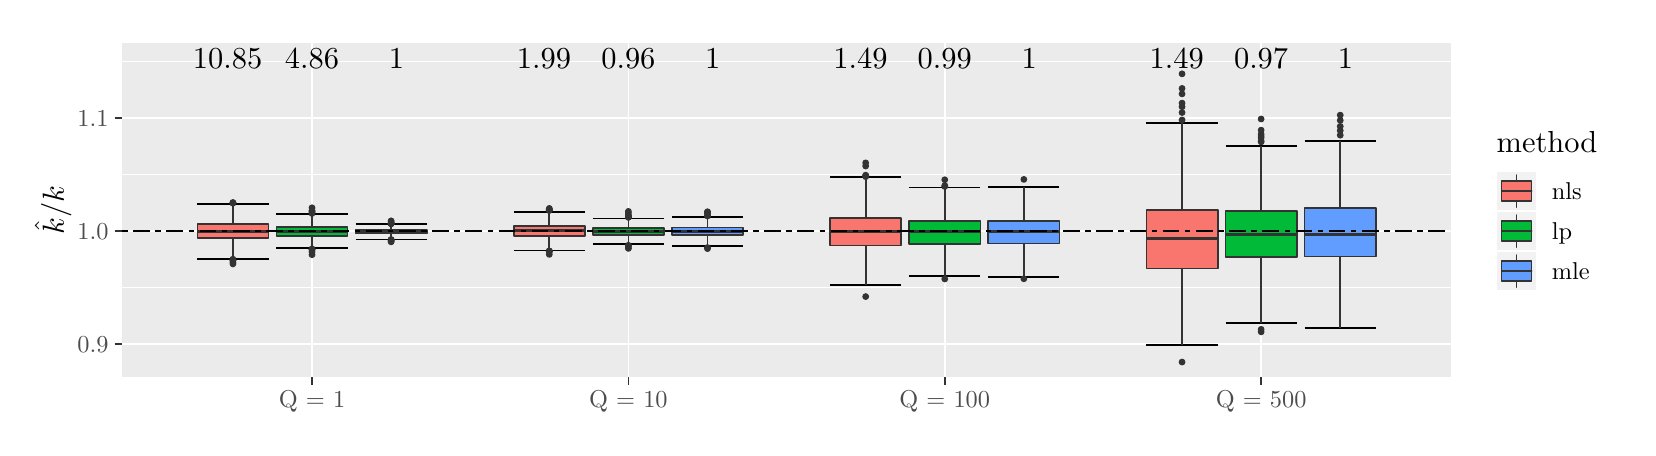
\begin{tikzpicture}[x=1pt,y=1pt]
\definecolor{fillColor}{RGB}{255,255,255}
\path[use as bounding box,fill=fillColor,fill opacity=0.00] (0,0) rectangle (578.16,144.54);
\begin{scope}
\path[clip] (  0.00,  0.00) rectangle (578.16,144.54);
\definecolor{drawColor}{RGB}{255,255,255}
\definecolor{fillColor}{RGB}{255,255,255}

\path[draw=drawColor,line width= 0.6pt,line join=round,line cap=round,fill=fillColor] (  0.00,  0.00) rectangle (578.16,144.54);
\end{scope}
\begin{scope}
\path[clip] ( 34.16, 18.22) rectangle (514.31,139.04);
\definecolor{fillColor}{gray}{0.92}

\path[fill=fillColor] ( 34.16, 18.22) rectangle (514.31,139.04);
\definecolor{drawColor}{RGB}{255,255,255}

\path[draw=drawColor,line width= 0.3pt,line join=round] ( 34.16, 50.58) --
	(514.31, 50.58);

\path[draw=drawColor,line width= 0.3pt,line join=round] ( 34.16, 91.38) --
	(514.31, 91.38);

\path[draw=drawColor,line width= 0.3pt,line join=round] ( 34.16,132.18) --
	(514.31,132.18);

\path[draw=drawColor,line width= 0.6pt,line join=round] ( 34.16, 30.18) --
	(514.31, 30.18);

\path[draw=drawColor,line width= 0.6pt,line join=round] ( 34.16, 70.98) --
	(514.31, 70.98);

\path[draw=drawColor,line width= 0.6pt,line join=round] ( 34.16,111.78) --
	(514.31,111.78);

\path[draw=drawColor,line width= 0.6pt,line join=round] (102.75, 18.22) --
	(102.75,139.04);

\path[draw=drawColor,line width= 0.6pt,line join=round] (217.07, 18.22) --
	(217.07,139.04);

\path[draw=drawColor,line width= 0.6pt,line join=round] (331.39, 18.22) --
	(331.39,139.04);

\path[draw=drawColor,line width= 0.6pt,line join=round] (445.71, 18.22) --
	(445.71,139.04);
\definecolor{drawColor}{RGB}{0,0,0}

\path[draw=drawColor,line width= 0.6pt,line join=round] ( 61.31, 80.94) --
	( 87.03, 80.94);

\path[draw=drawColor,line width= 0.6pt,line join=round] ( 74.17, 80.94) --
	( 74.17, 61.06);

\path[draw=drawColor,line width= 0.6pt,line join=round] ( 61.31, 61.06) --
	( 87.03, 61.06);

\path[draw=drawColor,line width= 0.6pt,line join=round] ( 89.89, 77.11) --
	(115.61, 77.11);

\path[draw=drawColor,line width= 0.6pt,line join=round] (102.75, 77.11) --
	(102.75, 64.89);

\path[draw=drawColor,line width= 0.6pt,line join=round] ( 89.89, 64.89) --
	(115.61, 64.89);

\path[draw=drawColor,line width= 0.6pt,line join=round] (118.47, 73.67) --
	(144.19, 73.67);

\path[draw=drawColor,line width= 0.6pt,line join=round] (131.33, 73.67) --
	(131.33, 68.00);

\path[draw=drawColor,line width= 0.6pt,line join=round] (118.47, 68.00) --
	(144.19, 68.00);

\path[draw=drawColor,line width= 0.6pt,line join=round] (175.63, 77.87) --
	(201.35, 77.87);

\path[draw=drawColor,line width= 0.6pt,line join=round] (188.49, 77.87) --
	(188.49, 64.00);

\path[draw=drawColor,line width= 0.6pt,line join=round] (175.63, 64.00) --
	(201.35, 64.00);

\path[draw=drawColor,line width= 0.6pt,line join=round] (204.21, 75.63) --
	(229.93, 75.63);

\path[draw=drawColor,line width= 0.6pt,line join=round] (217.07, 75.63) --
	(217.07, 66.36);

\path[draw=drawColor,line width= 0.6pt,line join=round] (204.21, 66.36) --
	(229.93, 66.36);

\path[draw=drawColor,line width= 0.6pt,line join=round] (232.79, 76.08) --
	(258.51, 76.08);

\path[draw=drawColor,line width= 0.6pt,line join=round] (245.65, 76.08) --
	(245.65, 65.75);

\path[draw=drawColor,line width= 0.6pt,line join=round] (232.79, 65.75) --
	(258.51, 65.75);

\path[draw=drawColor,line width= 0.6pt,line join=round] (289.95, 90.51) --
	(315.67, 90.51);

\path[draw=drawColor,line width= 0.6pt,line join=round] (302.81, 90.51) --
	(302.81, 51.44);

\path[draw=drawColor,line width= 0.6pt,line join=round] (289.95, 51.44) --
	(315.67, 51.44);

\path[draw=drawColor,line width= 0.6pt,line join=round] (318.53, 86.80) --
	(344.25, 86.80);

\path[draw=drawColor,line width= 0.6pt,line join=round] (331.39, 86.80) --
	(331.39, 54.85);

\path[draw=drawColor,line width= 0.6pt,line join=round] (318.53, 54.85) --
	(344.25, 54.85);

\path[draw=drawColor,line width= 0.6pt,line join=round] (347.11, 86.85) --
	(372.83, 86.85);

\path[draw=drawColor,line width= 0.6pt,line join=round] (359.97, 86.85) --
	(359.97, 54.35);

\path[draw=drawColor,line width= 0.6pt,line join=round] (347.11, 54.35) --
	(372.83, 54.35);

\path[draw=drawColor,line width= 0.6pt,line join=round] (404.27,110.08) --
	(430.00,110.08);

\path[draw=drawColor,line width= 0.6pt,line join=round] (417.13,110.08) --
	(417.13, 29.94);

\path[draw=drawColor,line width= 0.6pt,line join=round] (404.27, 29.94) --
	(430.00, 29.94);

\path[draw=drawColor,line width= 0.6pt,line join=round] (432.85,101.81) --
	(458.58,101.81);

\path[draw=drawColor,line width= 0.6pt,line join=round] (445.71,101.81) --
	(445.71, 37.90);

\path[draw=drawColor,line width= 0.6pt,line join=round] (432.85, 37.90) --
	(458.58, 37.90);

\path[draw=drawColor,line width= 0.6pt,line join=round] (461.43,103.50) --
	(487.16,103.50);

\path[draw=drawColor,line width= 0.6pt,line join=round] (474.29,103.50) --
	(474.29, 35.93);

\path[draw=drawColor,line width= 0.6pt,line join=round] (461.43, 35.93) --
	(487.16, 35.93);
\definecolor{drawColor}{gray}{0.20}
\definecolor{fillColor}{gray}{0.20}

\path[draw=drawColor,line width= 0.4pt,line join=round,line cap=round,fill=fillColor] ( 74.17, 81.13) circle (  1.02);

\path[draw=drawColor,line width= 0.4pt,line join=round,line cap=round,fill=fillColor] ( 74.17, 60.50) circle (  1.02);

\path[draw=drawColor,line width= 0.4pt,line join=round,line cap=round,fill=fillColor] ( 74.17, 81.21) circle (  1.02);

\path[draw=drawColor,line width= 0.4pt,line join=round,line cap=round,fill=fillColor] ( 74.17, 81.36) circle (  1.02);

\path[draw=drawColor,line width= 0.4pt,line join=round,line cap=round,fill=fillColor] ( 74.17, 59.17) circle (  1.02);

\path[draw=drawColor,line width= 0.4pt,line join=round,line cap=round,fill=fillColor] ( 74.17, 60.87) circle (  1.02);

\path[draw=drawColor,line width= 0.4pt,line join=round,line cap=round,fill=fillColor] ( 74.17, 59.75) circle (  1.02);

\path[draw=drawColor,line width= 0.4pt,line join=round,line cap=round,fill=fillColor] ( 74.17, 60.53) circle (  1.02);

\path[draw=drawColor,line width= 0.6pt,line join=round] ( 74.17, 73.48) -- ( 74.17, 80.94);

\path[draw=drawColor,line width= 0.6pt,line join=round] ( 74.17, 68.49) -- ( 74.17, 61.06);
\definecolor{fillColor}{RGB}{248,118,109}

\path[draw=drawColor,line width= 0.6pt,line join=round,line cap=round,fill=fillColor] ( 61.31, 73.48) --
	( 61.31, 68.49) --
	( 87.03, 68.49) --
	( 87.03, 73.48) --
	( 61.31, 73.48) --
	cycle;

\path[draw=drawColor,line width= 1.1pt,line join=round] ( 61.31, 70.99) -- ( 87.03, 70.99);
\definecolor{fillColor}{gray}{0.20}

\path[draw=drawColor,line width= 0.4pt,line join=round,line cap=round,fill=fillColor] (102.75, 62.50) circle (  1.02);

\path[draw=drawColor,line width= 0.4pt,line join=round,line cap=round,fill=fillColor] (102.75, 79.45) circle (  1.02);

\path[draw=drawColor,line width= 0.4pt,line join=round,line cap=round,fill=fillColor] (102.75, 77.40) circle (  1.02);

\path[draw=drawColor,line width= 0.4pt,line join=round,line cap=round,fill=fillColor] (102.75, 64.37) circle (  1.02);

\path[draw=drawColor,line width= 0.4pt,line join=round,line cap=round,fill=fillColor] (102.75, 77.81) circle (  1.02);

\path[draw=drawColor,line width= 0.4pt,line join=round,line cap=round,fill=fillColor] (102.75, 63.46) circle (  1.02);

\path[draw=drawColor,line width= 0.4pt,line join=round,line cap=round,fill=fillColor] (102.75, 78.10) circle (  1.02);

\path[draw=drawColor,line width= 0.4pt,line join=round,line cap=round,fill=fillColor] (102.75, 78.46) circle (  1.02);

\path[draw=drawColor,line width= 0.4pt,line join=round,line cap=round,fill=fillColor] (102.75, 64.61) circle (  1.02);

\path[draw=drawColor,line width= 0.4pt,line join=round,line cap=round,fill=fillColor] (102.75, 64.29) circle (  1.02);

\path[draw=drawColor,line width= 0.6pt,line join=round] (102.75, 72.48) -- (102.75, 77.11);

\path[draw=drawColor,line width= 0.6pt,line join=round] (102.75, 69.37) -- (102.75, 64.89);
\definecolor{fillColor}{RGB}{0,186,56}

\path[draw=drawColor,line width= 0.6pt,line join=round,line cap=round,fill=fillColor] ( 89.89, 72.48) --
	( 89.89, 69.37) --
	(115.61, 69.37) --
	(115.61, 72.48) --
	( 89.89, 72.48) --
	cycle;

\path[draw=drawColor,line width= 1.1pt,line join=round] ( 89.89, 70.99) -- (115.61, 70.99);
\definecolor{fillColor}{gray}{0.20}

\path[draw=drawColor,line width= 0.4pt,line join=round,line cap=round,fill=fillColor] (131.33, 74.66) circle (  1.02);

\path[draw=drawColor,line width= 0.4pt,line join=round,line cap=round,fill=fillColor] (131.33, 67.15) circle (  1.02);

\path[draw=drawColor,line width= 0.4pt,line join=round,line cap=round,fill=fillColor] (131.33, 73.84) circle (  1.02);

\path[draw=drawColor,line width= 0.4pt,line join=round,line cap=round,fill=fillColor] (131.33, 73.91) circle (  1.02);

\path[draw=drawColor,line width= 0.4pt,line join=round,line cap=round,fill=fillColor] (131.33, 74.69) circle (  1.02);

\path[draw=drawColor,line width= 0.4pt,line join=round,line cap=round,fill=fillColor] (131.33, 73.72) circle (  1.02);

\path[draw=drawColor,line width= 0.4pt,line join=round,line cap=round,fill=fillColor] (131.33, 67.87) circle (  1.02);

\path[draw=drawColor,line width= 0.4pt,line join=round,line cap=round,fill=fillColor] (131.33, 73.77) circle (  1.02);

\path[draw=drawColor,line width= 0.4pt,line join=round,line cap=round,fill=fillColor] (131.33, 67.96) circle (  1.02);

\path[draw=drawColor,line width= 0.4pt,line join=round,line cap=round,fill=fillColor] (131.33, 73.80) circle (  1.02);

\path[draw=drawColor,line width= 0.4pt,line join=round,line cap=round,fill=fillColor] (131.33, 73.72) circle (  1.02);

\path[draw=drawColor,line width= 0.4pt,line join=round,line cap=round,fill=fillColor] (131.33, 67.84) circle (  1.02);

\path[draw=drawColor,line width= 0.4pt,line join=round,line cap=round,fill=fillColor] (131.33, 67.65) circle (  1.02);

\path[draw=drawColor,line width= 0.4pt,line join=round,line cap=round,fill=fillColor] (131.33, 67.34) circle (  1.02);

\path[draw=drawColor,line width= 0.6pt,line join=round] (131.33, 71.54) -- (131.33, 73.67);

\path[draw=drawColor,line width= 0.6pt,line join=round] (131.33, 70.11) -- (131.33, 68.00);
\definecolor{fillColor}{RGB}{97,156,255}

\path[draw=drawColor,line width= 0.6pt,line join=round,line cap=round,fill=fillColor] (118.47, 71.54) --
	(118.47, 70.11) --
	(144.19, 70.11) --
	(144.19, 71.54) --
	(118.47, 71.54) --
	cycle;

\path[draw=drawColor,line width= 1.1pt,line join=round] (118.47, 70.84) -- (144.19, 70.84);
\definecolor{fillColor}{gray}{0.20}

\path[draw=drawColor,line width= 0.4pt,line join=round,line cap=round,fill=fillColor] (188.49, 62.61) circle (  1.02);

\path[draw=drawColor,line width= 0.4pt,line join=round,line cap=round,fill=fillColor] (188.49, 78.74) circle (  1.02);

\path[draw=drawColor,line width= 0.4pt,line join=round,line cap=round,fill=fillColor] (188.49, 78.67) circle (  1.02);

\path[draw=drawColor,line width= 0.4pt,line join=round,line cap=round,fill=fillColor] (188.49, 63.85) circle (  1.02);

\path[draw=drawColor,line width= 0.4pt,line join=round,line cap=round,fill=fillColor] (188.49, 78.86) circle (  1.02);

\path[draw=drawColor,line width= 0.4pt,line join=round,line cap=round,fill=fillColor] (188.49, 63.70) circle (  1.02);

\path[draw=drawColor,line width= 0.4pt,line join=round,line cap=round,fill=fillColor] (188.49, 63.74) circle (  1.02);

\path[draw=drawColor,line width= 0.4pt,line join=round,line cap=round,fill=fillColor] (188.49, 63.79) circle (  1.02);

\path[draw=drawColor,line width= 0.4pt,line join=round,line cap=round,fill=fillColor] (188.49, 79.23) circle (  1.02);

\path[draw=drawColor,line width= 0.4pt,line join=round,line cap=round,fill=fillColor] (188.49, 78.48) circle (  1.02);

\path[draw=drawColor,line width= 0.6pt,line join=round] (188.49, 72.87) -- (188.49, 77.87);

\path[draw=drawColor,line width= 0.6pt,line join=round] (188.49, 69.27) -- (188.49, 64.00);
\definecolor{fillColor}{RGB}{248,118,109}

\path[draw=drawColor,line width= 0.6pt,line join=round,line cap=round,fill=fillColor] (175.63, 72.87) --
	(175.63, 69.27) --
	(201.35, 69.27) --
	(201.35, 72.87) --
	(175.63, 72.87) --
	cycle;

\path[draw=drawColor,line width= 1.1pt,line join=round] (175.63, 71.12) -- (201.35, 71.12);
\definecolor{fillColor}{gray}{0.20}

\path[draw=drawColor,line width= 0.4pt,line join=round,line cap=round,fill=fillColor] (217.07, 65.74) circle (  1.02);

\path[draw=drawColor,line width= 0.4pt,line join=round,line cap=round,fill=fillColor] (217.07, 76.51) circle (  1.02);

\path[draw=drawColor,line width= 0.4pt,line join=round,line cap=round,fill=fillColor] (217.07, 76.05) circle (  1.02);

\path[draw=drawColor,line width= 0.4pt,line join=round,line cap=round,fill=fillColor] (217.07, 65.87) circle (  1.02);

\path[draw=drawColor,line width= 0.4pt,line join=round,line cap=round,fill=fillColor] (217.07, 76.17) circle (  1.02);

\path[draw=drawColor,line width= 0.4pt,line join=round,line cap=round,fill=fillColor] (217.07, 77.59) circle (  1.02);

\path[draw=drawColor,line width= 0.4pt,line join=round,line cap=round,fill=fillColor] (217.07, 76.08) circle (  1.02);

\path[draw=drawColor,line width= 0.4pt,line join=round,line cap=round,fill=fillColor] (217.07, 64.81) circle (  1.02);

\path[draw=drawColor,line width= 0.4pt,line join=round,line cap=round,fill=fillColor] (217.07, 76.09) circle (  1.02);

\path[draw=drawColor,line width= 0.4pt,line join=round,line cap=round,fill=fillColor] (217.07, 76.36) circle (  1.02);

\path[draw=drawColor,line width= 0.4pt,line join=round,line cap=round,fill=fillColor] (217.07, 65.78) circle (  1.02);

\path[draw=drawColor,line width= 0.4pt,line join=round,line cap=round,fill=fillColor] (217.07, 64.87) circle (  1.02);

\path[draw=drawColor,line width= 0.4pt,line join=round,line cap=round,fill=fillColor] (217.07, 76.82) circle (  1.02);

\path[draw=drawColor,line width= 0.4pt,line join=round,line cap=round,fill=fillColor] (217.07, 78.16) circle (  1.02);

\path[draw=drawColor,line width= 0.6pt,line join=round] (217.07, 72.23) -- (217.07, 75.63);

\path[draw=drawColor,line width= 0.6pt,line join=round] (217.07, 69.73) -- (217.07, 66.36);
\definecolor{fillColor}{RGB}{0,186,56}

\path[draw=drawColor,line width= 0.6pt,line join=round,line cap=round,fill=fillColor] (204.21, 72.23) --
	(204.21, 69.73) --
	(229.93, 69.73) --
	(229.93, 72.23) --
	(204.21, 72.23) --
	cycle;

\path[draw=drawColor,line width= 1.1pt,line join=round] (204.21, 70.94) -- (229.93, 70.94);
\definecolor{fillColor}{gray}{0.20}

\path[draw=drawColor,line width= 0.4pt,line join=round,line cap=round,fill=fillColor] (245.65, 78.02) circle (  1.02);

\path[draw=drawColor,line width= 0.4pt,line join=round,line cap=round,fill=fillColor] (245.65, 64.70) circle (  1.02);

\path[draw=drawColor,line width= 0.4pt,line join=round,line cap=round,fill=fillColor] (245.65, 76.50) circle (  1.02);

\path[draw=drawColor,line width= 0.4pt,line join=round,line cap=round,fill=fillColor] (245.65, 76.62) circle (  1.02);

\path[draw=drawColor,line width= 0.4pt,line join=round,line cap=round,fill=fillColor] (245.65, 65.10) circle (  1.02);

\path[draw=drawColor,line width= 0.4pt,line join=round,line cap=round,fill=fillColor] (245.65, 77.32) circle (  1.02);

\path[draw=drawColor,line width= 0.4pt,line join=round,line cap=round,fill=fillColor] (245.65, 77.89) circle (  1.02);

\path[draw=drawColor,line width= 0.6pt,line join=round] (245.65, 72.31) -- (245.65, 76.08);

\path[draw=drawColor,line width= 0.6pt,line join=round] (245.65, 69.68) -- (245.65, 65.75);
\definecolor{fillColor}{RGB}{97,156,255}

\path[draw=drawColor,line width= 0.6pt,line join=round,line cap=round,fill=fillColor] (232.79, 72.31) --
	(232.79, 69.68) --
	(258.51, 69.68) --
	(258.51, 72.31) --
	(232.79, 72.31) --
	cycle;

\path[draw=drawColor,line width= 1.1pt,line join=round] (232.79, 70.97) -- (258.51, 70.97);
\definecolor{fillColor}{gray}{0.20}

\path[draw=drawColor,line width= 0.4pt,line join=round,line cap=round,fill=fillColor] (302.81, 94.56) circle (  1.02);

\path[draw=drawColor,line width= 0.4pt,line join=round,line cap=round,fill=fillColor] (302.81, 90.97) circle (  1.02);

\path[draw=drawColor,line width= 0.4pt,line join=round,line cap=round,fill=fillColor] (302.81, 90.70) circle (  1.02);

\path[draw=drawColor,line width= 0.4pt,line join=round,line cap=round,fill=fillColor] (302.81, 91.23) circle (  1.02);

\path[draw=drawColor,line width= 0.4pt,line join=round,line cap=round,fill=fillColor] (302.81, 90.95) circle (  1.02);

\path[draw=drawColor,line width= 0.4pt,line join=round,line cap=round,fill=fillColor] (302.81, 47.37) circle (  1.02);

\path[draw=drawColor,line width= 0.4pt,line join=round,line cap=round,fill=fillColor] (302.81, 95.69) circle (  1.02);

\path[draw=drawColor,line width= 0.6pt,line join=round] (302.81, 75.76) -- (302.81, 90.51);

\path[draw=drawColor,line width= 0.6pt,line join=round] (302.81, 65.88) -- (302.81, 51.44);
\definecolor{fillColor}{RGB}{248,118,109}

\path[draw=drawColor,line width= 0.6pt,line join=round,line cap=round,fill=fillColor] (289.95, 75.76) --
	(289.95, 65.88) --
	(315.67, 65.88) --
	(315.67, 75.76) --
	(289.95, 75.76) --
	cycle;

\path[draw=drawColor,line width= 1.1pt,line join=round] (289.95, 70.82) -- (315.67, 70.82);
\definecolor{fillColor}{gray}{0.20}

\path[draw=drawColor,line width= 0.4pt,line join=round,line cap=round,fill=fillColor] (331.39, 53.74) circle (  1.02);

\path[draw=drawColor,line width= 0.4pt,line join=round,line cap=round,fill=fillColor] (331.39, 87.47) circle (  1.02);

\path[draw=drawColor,line width= 0.4pt,line join=round,line cap=round,fill=fillColor] (331.39, 87.17) circle (  1.02);

\path[draw=drawColor,line width= 0.4pt,line join=round,line cap=round,fill=fillColor] (331.39, 89.58) circle (  1.02);

\path[draw=drawColor,line width= 0.6pt,line join=round] (331.39, 74.61) -- (331.39, 86.80);

\path[draw=drawColor,line width= 0.6pt,line join=round] (331.39, 66.47) -- (331.39, 54.85);
\definecolor{fillColor}{RGB}{0,186,56}

\path[draw=drawColor,line width= 0.6pt,line join=round,line cap=round,fill=fillColor] (318.53, 74.61) --
	(318.53, 66.47) --
	(344.25, 66.47) --
	(344.25, 74.61) --
	(318.53, 74.61) --
	cycle;

\path[draw=drawColor,line width= 1.1pt,line join=round] (318.53, 70.90) -- (344.25, 70.90);
\definecolor{fillColor}{gray}{0.20}

\path[draw=drawColor,line width= 0.4pt,line join=round,line cap=round,fill=fillColor] (359.97, 89.71) circle (  1.02);

\path[draw=drawColor,line width= 0.4pt,line join=round,line cap=round,fill=fillColor] (359.97, 53.80) circle (  1.02);

\path[draw=drawColor,line width= 0.6pt,line join=round] (359.97, 74.76) -- (359.97, 86.85);

\path[draw=drawColor,line width= 0.6pt,line join=round] (359.97, 66.54) -- (359.97, 54.35);
\definecolor{fillColor}{RGB}{97,156,255}

\path[draw=drawColor,line width= 0.6pt,line join=round,line cap=round,fill=fillColor] (347.11, 74.76) --
	(347.11, 66.54) --
	(372.83, 66.54) --
	(372.83, 74.76) --
	(347.11, 74.76) --
	cycle;

\path[draw=drawColor,line width= 1.1pt,line join=round] (347.11, 70.81) -- (372.83, 70.81);
\definecolor{fillColor}{gray}{0.20}

\path[draw=drawColor,line width= 0.4pt,line join=round,line cap=round,fill=fillColor] (417.13,117.28) circle (  1.02);

\path[draw=drawColor,line width= 0.4pt,line join=round,line cap=round,fill=fillColor] (417.13,111.18) circle (  1.02);

\path[draw=drawColor,line width= 0.4pt,line join=round,line cap=round,fill=fillColor] (417.13,122.59) circle (  1.02);

\path[draw=drawColor,line width= 0.4pt,line join=round,line cap=round,fill=fillColor] (417.13,113.87) circle (  1.02);

\path[draw=drawColor,line width= 0.4pt,line join=round,line cap=round,fill=fillColor] (417.13, 23.71) circle (  1.02);

\path[draw=drawColor,line width= 0.4pt,line join=round,line cap=round,fill=fillColor] (417.13,120.61) circle (  1.02);

\path[draw=drawColor,line width= 0.4pt,line join=round,line cap=round,fill=fillColor] (417.13,127.86) circle (  1.02);

\path[draw=drawColor,line width= 0.4pt,line join=round,line cap=round,fill=fillColor] (417.13,115.96) circle (  1.02);

\path[draw=drawColor,line width= 0.6pt,line join=round] (417.13, 78.75) -- (417.13,110.08);

\path[draw=drawColor,line width= 0.6pt,line join=round] (417.13, 57.52) -- (417.13, 29.94);
\definecolor{fillColor}{RGB}{248,118,109}

\path[draw=drawColor,line width= 0.6pt,line join=round,line cap=round,fill=fillColor] (404.27, 78.75) --
	(404.27, 57.52) --
	(430.00, 57.52) --
	(430.00, 78.75) --
	(404.27, 78.75) --
	cycle;

\path[draw=drawColor,line width= 1.1pt,line join=round] (404.27, 68.30) -- (430.00, 68.30);
\definecolor{fillColor}{gray}{0.20}

\path[draw=drawColor,line width= 0.4pt,line join=round,line cap=round,fill=fillColor] (445.71,105.37) circle (  1.02);

\path[draw=drawColor,line width= 0.4pt,line join=round,line cap=round,fill=fillColor] (445.71,106.09) circle (  1.02);

\path[draw=drawColor,line width= 0.4pt,line join=round,line cap=round,fill=fillColor] (445.71,107.52) circle (  1.02);

\path[draw=drawColor,line width= 0.4pt,line join=round,line cap=round,fill=fillColor] (445.71,111.54) circle (  1.02);

\path[draw=drawColor,line width= 0.4pt,line join=round,line cap=round,fill=fillColor] (445.71, 35.53) circle (  1.02);

\path[draw=drawColor,line width= 0.4pt,line join=round,line cap=round,fill=fillColor] (445.71,103.59) circle (  1.02);

\path[draw=drawColor,line width= 0.4pt,line join=round,line cap=round,fill=fillColor] (445.71,103.27) circle (  1.02);

\path[draw=drawColor,line width= 0.4pt,line join=round,line cap=round,fill=fillColor] (445.71, 34.62) circle (  1.02);

\path[draw=drawColor,line width= 0.4pt,line join=round,line cap=round,fill=fillColor] (445.71,104.75) circle (  1.02);

\path[draw=drawColor,line width= 0.6pt,line join=round] (445.71, 78.35) -- (445.71,101.81);

\path[draw=drawColor,line width= 0.6pt,line join=round] (445.71, 61.79) -- (445.71, 37.90);
\definecolor{fillColor}{RGB}{0,186,56}

\path[draw=drawColor,line width= 0.6pt,line join=round,line cap=round,fill=fillColor] (432.85, 78.35) --
	(432.85, 61.79) --
	(458.58, 61.79) --
	(458.58, 78.35) --
	(432.85, 78.35) --
	cycle;

\path[draw=drawColor,line width= 1.1pt,line join=round] (432.85, 69.74) -- (458.58, 69.74);
\definecolor{fillColor}{gray}{0.20}

\path[draw=drawColor,line width= 0.4pt,line join=round,line cap=round,fill=fillColor] (474.29,105.69) circle (  1.02);

\path[draw=drawColor,line width= 0.4pt,line join=round,line cap=round,fill=fillColor] (474.29,108.87) circle (  1.02);

\path[draw=drawColor,line width= 0.4pt,line join=round,line cap=round,fill=fillColor] (474.29,111.06) circle (  1.02);

\path[draw=drawColor,line width= 0.4pt,line join=round,line cap=round,fill=fillColor] (474.29,112.94) circle (  1.02);

\path[draw=drawColor,line width= 0.4pt,line join=round,line cap=round,fill=fillColor] (474.29,107.35) circle (  1.02);

\path[draw=drawColor,line width= 0.6pt,line join=round] (474.29, 79.32) -- (474.29,103.50);

\path[draw=drawColor,line width= 0.6pt,line join=round] (474.29, 61.85) -- (474.29, 35.93);
\definecolor{fillColor}{RGB}{97,156,255}

\path[draw=drawColor,line width= 0.6pt,line join=round,line cap=round,fill=fillColor] (461.43, 79.32) --
	(461.43, 61.85) --
	(487.16, 61.85) --
	(487.16, 79.32) --
	(461.43, 79.32) --
	cycle;

\path[draw=drawColor,line width= 1.1pt,line join=round] (461.43, 69.81) -- (487.16, 69.81);
\definecolor{drawColor}{RGB}{0,0,0}

\path[draw=drawColor,line width= 0.6pt,dash pattern=on 2pt off 2pt on 6pt off 2pt ,line join=round] ( 34.16, 70.98) -- (514.31, 70.98);

\node[text=drawColor,anchor=base,inner sep=0pt, outer sep=0pt, scale=  1.10] at (133.23,129.75) {1};

\node[text=drawColor,anchor=base,inner sep=0pt, outer sep=0pt, scale=  1.10] at (102.75,129.75) {4.86};

\node[text=drawColor,anchor=base,inner sep=0pt, outer sep=0pt, scale=  1.10] at ( 72.26,129.75) {10.85};

\node[text=drawColor,anchor=base,inner sep=0pt, outer sep=0pt, scale=  1.10] at (247.56,129.75) {1};

\node[text=drawColor,anchor=base,inner sep=0pt, outer sep=0pt, scale=  1.10] at (217.07,129.75) {0.96};

\node[text=drawColor,anchor=base,inner sep=0pt, outer sep=0pt, scale=  1.10] at (186.59,129.75) {1.99};

\node[text=drawColor,anchor=base,inner sep=0pt, outer sep=0pt, scale=  1.10] at (361.88,129.75) {1};

\node[text=drawColor,anchor=base,inner sep=0pt, outer sep=0pt, scale=  1.10] at (331.39,129.75) {0.99};

\node[text=drawColor,anchor=base,inner sep=0pt, outer sep=0pt, scale=  1.10] at (300.91,129.75) {1.49};

\node[text=drawColor,anchor=base,inner sep=0pt, outer sep=0pt, scale=  1.10] at (476.20,129.75) {1};

\node[text=drawColor,anchor=base,inner sep=0pt, outer sep=0pt, scale=  1.10] at (445.71,129.75) {0.97};

\node[text=drawColor,anchor=base,inner sep=0pt, outer sep=0pt, scale=  1.10] at (415.23,129.75) {1.49};
\end{scope}
\begin{scope}
\path[clip] (  0.00,  0.00) rectangle (578.16,144.54);
\definecolor{drawColor}{gray}{0.30}

\node[text=drawColor,anchor=base east,inner sep=0pt, outer sep=0pt, scale=  0.88] at ( 29.21, 27.15) {0.9};

\node[text=drawColor,anchor=base east,inner sep=0pt, outer sep=0pt, scale=  0.88] at ( 29.21, 67.95) {1.0};

\node[text=drawColor,anchor=base east,inner sep=0pt, outer sep=0pt, scale=  0.88] at ( 29.21,108.75) {1.1};
\end{scope}
\begin{scope}
\path[clip] (  0.00,  0.00) rectangle (578.16,144.54);
\definecolor{drawColor}{gray}{0.20}

\path[draw=drawColor,line width= 0.6pt,line join=round] ( 31.41, 30.18) --
	( 34.16, 30.18);

\path[draw=drawColor,line width= 0.6pt,line join=round] ( 31.41, 70.98) --
	( 34.16, 70.98);

\path[draw=drawColor,line width= 0.6pt,line join=round] ( 31.41,111.78) --
	( 34.16,111.78);
\end{scope}
\begin{scope}
\path[clip] (  0.00,  0.00) rectangle (578.16,144.54);
\definecolor{drawColor}{gray}{0.20}

\path[draw=drawColor,line width= 0.6pt,line join=round] (102.75, 15.47) --
	(102.75, 18.22);

\path[draw=drawColor,line width= 0.6pt,line join=round] (217.07, 15.47) --
	(217.07, 18.22);

\path[draw=drawColor,line width= 0.6pt,line join=round] (331.39, 15.47) --
	(331.39, 18.22);

\path[draw=drawColor,line width= 0.6pt,line join=round] (445.71, 15.47) --
	(445.71, 18.22);
\end{scope}
\begin{scope}
\path[clip] (  0.00,  0.00) rectangle (578.16,144.54);
\definecolor{drawColor}{gray}{0.30}

\node[text=drawColor,anchor=base,inner sep=0pt, outer sep=0pt, scale=  0.88] at (102.75,  7.21) {Q = 1};

\node[text=drawColor,anchor=base,inner sep=0pt, outer sep=0pt, scale=  0.88] at (217.07,  7.21) {Q = 10};

\node[text=drawColor,anchor=base,inner sep=0pt, outer sep=0pt, scale=  0.88] at (331.39,  7.21) {Q = 100};

\node[text=drawColor,anchor=base,inner sep=0pt, outer sep=0pt, scale=  0.88] at (445.71,  7.21) {Q = 500};
\end{scope}
\begin{scope}
\path[clip] (  0.00,  0.00) rectangle (578.16,144.54);
\definecolor{drawColor}{RGB}{0,0,0}

\node[text=drawColor,rotate= 90.00,anchor=base,inner sep=0pt, outer sep=0pt, scale=  1.10] at ( 13.08, 78.63) {$\hat{k}/k$};
\end{scope}
\begin{scope}
\path[clip] (  0.00,  0.00) rectangle (578.16,144.54);
\definecolor{fillColor}{RGB}{255,255,255}

\path[fill=fillColor] (525.31, 43.84) rectangle (572.66,113.42);
\end{scope}
\begin{scope}
\path[clip] (  0.00,  0.00) rectangle (578.16,144.54);
\definecolor{drawColor}{RGB}{0,0,0}

\node[text=drawColor,anchor=base west,inner sep=0pt, outer sep=0pt, scale=  1.10] at (530.81, 99.27) {method};
\end{scope}
\begin{scope}
\path[clip] (  0.00,  0.00) rectangle (578.16,144.54);
\definecolor{drawColor}{RGB}{255,255,255}
\definecolor{fillColor}{gray}{0.95}

\path[draw=drawColor,line width= 0.6pt,line join=round,line cap=round,fill=fillColor] (530.81, 78.25) rectangle (545.26, 92.70);
\end{scope}
\begin{scope}
\path[clip] (  0.00,  0.00) rectangle (578.16,144.54);
\definecolor{drawColor}{gray}{0.20}

\path[draw=drawColor,line width= 0.6pt,line join=round,line cap=round] (538.03, 79.70) --
	(538.03, 81.86);

\path[draw=drawColor,line width= 0.6pt,line join=round,line cap=round] (538.03, 89.09) --
	(538.03, 91.26);
\definecolor{fillColor}{RGB}{248,118,109}

\path[draw=drawColor,line width= 0.6pt,line join=round,line cap=round,fill=fillColor] (532.61, 81.86) rectangle (543.45, 89.09);

\path[draw=drawColor,line width= 0.6pt,line join=round,line cap=round] (532.61, 85.48) --
	(543.45, 85.48);
\end{scope}
\begin{scope}
\path[clip] (  0.00,  0.00) rectangle (578.16,144.54);
\definecolor{drawColor}{RGB}{255,255,255}
\definecolor{fillColor}{gray}{0.95}

\path[draw=drawColor,line width= 0.6pt,line join=round,line cap=round,fill=fillColor] (530.81, 63.80) rectangle (545.26, 78.25);
\end{scope}
\begin{scope}
\path[clip] (  0.00,  0.00) rectangle (578.16,144.54);
\definecolor{drawColor}{gray}{0.20}

\path[draw=drawColor,line width= 0.6pt,line join=round,line cap=round] (538.03, 65.24) --
	(538.03, 67.41);

\path[draw=drawColor,line width= 0.6pt,line join=round,line cap=round] (538.03, 74.64) --
	(538.03, 76.81);
\definecolor{fillColor}{RGB}{0,186,56}

\path[draw=drawColor,line width= 0.6pt,line join=round,line cap=round,fill=fillColor] (532.61, 67.41) rectangle (543.45, 74.64);

\path[draw=drawColor,line width= 0.6pt,line join=round,line cap=round] (532.61, 71.02) --
	(543.45, 71.02);
\end{scope}
\begin{scope}
\path[clip] (  0.00,  0.00) rectangle (578.16,144.54);
\definecolor{drawColor}{RGB}{255,255,255}
\definecolor{fillColor}{gray}{0.95}

\path[draw=drawColor,line width= 0.6pt,line join=round,line cap=round,fill=fillColor] (530.81, 49.34) rectangle (545.26, 63.80);
\end{scope}
\begin{scope}
\path[clip] (  0.00,  0.00) rectangle (578.16,144.54);
\definecolor{drawColor}{gray}{0.20}

\path[draw=drawColor,line width= 0.6pt,line join=round,line cap=round] (538.03, 50.79) --
	(538.03, 52.96);

\path[draw=drawColor,line width= 0.6pt,line join=round,line cap=round] (538.03, 60.18) --
	(538.03, 62.35);
\definecolor{fillColor}{RGB}{97,156,255}

\path[draw=drawColor,line width= 0.6pt,line join=round,line cap=round,fill=fillColor] (532.61, 52.96) rectangle (543.45, 60.18);

\path[draw=drawColor,line width= 0.6pt,line join=round,line cap=round] (532.61, 56.57) --
	(543.45, 56.57);
\end{scope}
\begin{scope}
\path[clip] (  0.00,  0.00) rectangle (578.16,144.54);
\definecolor{drawColor}{RGB}{0,0,0}

\node[text=drawColor,anchor=base west,inner sep=0pt, outer sep=0pt, scale=  0.88] at (550.76, 82.45) {nls};
\end{scope}
\begin{scope}
\path[clip] (  0.00,  0.00) rectangle (578.16,144.54);
\definecolor{drawColor}{RGB}{0,0,0}

\node[text=drawColor,anchor=base west,inner sep=0pt, outer sep=0pt, scale=  0.88] at (550.76, 67.99) {lp};
\end{scope}
\begin{scope}
\path[clip] (  0.00,  0.00) rectangle (578.16,144.54);
\definecolor{drawColor}{RGB}{0,0,0}

\node[text=drawColor,anchor=base west,inner sep=0pt, outer sep=0pt, scale=  0.88] at (550.76, 53.54) {mle};
\end{scope}
\end{tikzpicture}
